\chapter{Mobiele HTML5-raamwerken}
\label{chap:raamwerken}

In dit hoofdstuk wordt ingezoomd op de mobiele HTML5-raamwerken die dit werk vergelijkt, namelijk \jqm{}~(\ref{sec:raamwerk-jqm}), \st{}~(\ref{sec:raamwerk-st}), \kendo{}~(\ref{sec:raamwerk-kendo}) en \lungo{}~(\ref{sec:raamwerk-lungo}).
In de laatste sectie (\ref{sec:raamwerken-tabel}) wordt een tabel weergegeven, waarin deze gegevens worden vergeleken.

\section{\jqm}
\label{sec:raamwerk-jqm}
\jqm{} is een opmaakgedreven raamwerk dat werd aangekondigd in 2010 en hoofdzakelijk gebruikersinterface-elementen (GI-elementen) aanbiedt~\cite{Resig2010}.
In november 2011 werd versie~1.0 uitgebracht~\cite{Parker2011} en een jaar later werd in oktober versie~1.2 uitgebracht~\cite{Parker2012}. 
Op het moment van schrijven zit \jqm{} aan versie~1.3.1~\cite{Parker2013b}. 
Het raamwerk wordt beheerd door het jQuery Project dat onder andere jQuery Core beheert en waar \jqm{} afhankelijk van is~\cite{JQuery2012}. 
\jqm{} wordt door onder andere Adobe, BlackBerry en Mozilla gesponsord~\cite{JQuery2012a}.

\subsection{Omkadering}
\paragraph{Programmeertaal}
Om met \jqm{} aan de slag te kunnen, is niets meer nodig dan kennis over HTML, CSS en \js{}. 
Alle GI-elementen worden geschreven in HTML en aangeduid met \code{data-}* attributen.

\paragraph{Tools}
Een standaard teksteditor voldoet om met \jqm{} aan de slag te kunnen. 
Natuurlijk kan het gemakkelijk zijn om van \term{integrated development environments}~(IDE's) zoals Aptana Studio~\cite{Aptana2012} of WebStorm~\cite{JetBrains2012} gebruik te maken, waardoor handige kenmerken zoals automatische code-aanvulling beschikbaar zijn.

Het is ook mogelijk om gebruik te maken van Codiqua om de GI-elementen op het scherm te slepen en neer te zetten. 
Codiqua zal automatisch op de achtergrond de HTML-code voorzien~\cite{Sperry2012}.

\paragraph{Documentatie}
Documentatie is te vinden op \exturl{www.jquerymobile.com/demos/1.2.0} voor versie~1.2. 
Hierop is een catalogus te vinden van alle mogelijke elementen waarover \jqm{} beschikt. 
Door de broncode van een voorbeeld te bekijken, kan worden gekeken welke code moet worden geschreven om tot dat resultaat te komen.

Naast de GI-elementen is er ook documentatie over de API. 
Deze gaat over initiële configuraties, \term{events} en methodes die kunnen worden gebruikt.

\paragraph{Marktadoptatie}
Op de website van \jqm{} wordt een reeks applicaties getoond die gemaakt zijn met hun raamwerk. 
Enkele voorbeelden zijn webapplicaties voor Ikea, Disney World, Stanford University en Moulin Rouge~\cite{JQuery2012a}. 

\paragraph{Licenties}
Sinds september 2012 is het enkel nog mogelijk om \jqm{} onder de Massachusetts Institute of Technology (MIT) licentie te verkrijgen~\cite{Dmethvin2012}. 
Dit betekent dat de code wordt vrijgegeven als \term{open-source} en dat deze tegelijkertijd kan worden gebruikt in propriëtaire projecten en applicaties~\cite{PhilDutson2012}.

\subsection{Code en ontwikkeling}
Zoals werd aangehaald, wordt voornamelijk HTML5-code geschreven voorzien van \code{data-}* attributen. 
Daarna zal het raamwerk door middel van \term{progressive enhancement} allerhande code toevoegen om de beoogde GI-elementen correct te tonen in de browser. 
Dit wordt verder uitgelegd in de sectie browserondersteuning (zie \ref{sec:jqm-browser-support}).

Er zijn drie strategieën om webapplicaties te maken in \jqm{}~\cite{Broulik2012}. 
Een eerste is om de volledige applicatie in één webpagina te schrijven. 
De vele schermen van de webapplicatie zijn dan allemaal samengebracht op eenzelfde webpagina. 
Het voordeel bij deze aanpak is dat er initieel minder verzoeken zijn naar de server omdat alles in één bestand wordt opgehaald. 
Dit geldt ook zo voor de geïmporteerde CSS- en \js{}-bestanden. 

Een tweede strategie is om voor ieder scherm een aparte webpagina aan te maken. 
Het voordeel hierbij is dat de eerste pagina waar de gebruiker op terecht komt, sneller wordt gedownload. 
Bij iedere navigatie naar een ander scherm, moet dit scherm via Asynchronous \js{} and XML~(AJAX) worden opgehaald, waardoor dit vertragend kan werken. 

Een laatste strategie is om een mix tussen beide te maken. 
Men kan bijvoorbeeld alle schermen die de gebruiker vaak nodig heeft op één webpagina plaatsen. 
De schermen die de gebruiker zelden nodig heeft, worden op aparte webpagina's geplaatst.   

\subsection{Functionele kenmerken}
\jqm{} is een raamwerk dat voornamelijk GI-elementen aanbiedt, met name pagina's en dialoogvensters, werkbalken, knoppen, inhoud vormgeven, elementen voor formulieren en lijsten~\cite{JQuery2012b}.
Deze kenmerken zijn gebaseerd op versie~1.2.

\begin{enumerate}
\item \textbf{Pagina's en dialoogvensters}
De basisstructuur van een pagina bestaat uit een koptekst, inhoud en voettekst. 
Bij het overgaan naar een andere pagina wordt gekozen uit tien overgangseffecten. 
Voordat deze overgang gebeurt, zal \jqm{} altijd eerst die pagina ophalen via AJAX en inladen in het DOM. 
Zo kan een soepel overgangseffect worden getoond aan de gebruiker. 
Daarnaast is het ook mogelijk om gelinkte pagina's op voorhand op te halen. 
Als laatste biedt \jqm{} ook dialoogvensters en pop-ups aan. 

\item \textbf{Werkbalken}
Het is mogelijk om zowel knoppen bij de koptekst als bij de voettekst te plaatsen. 
Bij deze laatste kunnen typisch meer knoppen geplaatst worden, bij de koptekst slechts twee. 
Daarnaast is het ook mogelijk om navigatiebalken te maken. 
Aan zowel de werk- als navigatiebalken kunnen iconen worden toegevoegd.

\item \textbf{Knoppen}
Het is ook mogelijk om knoppen te plaatsen in het inhoud gedeelde. 
Ook hier is er terug een variëteit aan mogelijkheden: grote of kleine, met iconen of zonder, gegroepeerd of niet. 

\item \textbf{Inhoud vormgeven}
De inhoud van de pagina kan worden vormgegeven door gebruik te maken van een rooster. 
\jqm{} laat roosters tot vijf kolommen toe. 
Daarnaast zijn er ook nog opklapbare blokken ter beschikking. 
Als laatste kunnen deze blokken ook samengevoegd worden tot een accordeon. 

\item \textbf{Elementen voor formulieren}
\jqm{} biedt alle gangbare elementen voor formulieren aan zoals tekstinvoer, een selectie uit een lijst, een zoekveld, een \term{slider} en een \term{switch}. 
Het raamwerk verplicht zelfs om de \code{<label>}-tag te gebruiken. 
Zo wordt de applicatie toegankelijker gemaakt voor bijvoorbeeld mensen met een \term{e-reader}.

\item \textbf{Lijsten}
Een laatste categorie GI-elementen die \jqm{} aanbiedt, zijn lijsten. 
Deze gaan van standaard ongeordende lijsten tot lijsten met alle soorten decoraties als iconen, afbeeldingen, telbubbels en verdelers. 
Ook is het mogelijk om in deze lijsten te zoeken. 
Hiervoor dient de gebruiker enkel één data attribuut toe te voegen, waarna het raamwerk de implementatie voorziet. 
\end{enumerate}

\subsection{Niet-functionele kenmerken}
\paragraph{Performantie}
Zoals gezegd schrijft de ontwikkelaar HTML5-code met specifieke data-attributen en zal het raamwerk daarna de code verder aanvullen. 
Dit gebeurt enkel op de pagina die de gebruiker op dat moment bekijkt. 
Dit gaat dus ook op voor een webapplicatie waarbij alle schermen op één webpagina zijn geschreven. 
Deze webpagina bevat allemaal \code{<div>}-verpakkingen voor ieder scherm. 
\jqm{} zal enkel die \code{<div>} verder aanvullen die op dat moment getoond wordt aan de gebruiker. 

\paragraph{Aanpasbaarheid}
Als \jqm{} \term{out-of-the-box} wordt gebruikt, zit alles al goed qua kleur en design. 
Er is keuze uit vijf kleurenthema's die kunnen worden toegepast op de gehele applicatie of enkel op bepaalde elementen. 
Om een applicatie echt te laten onderscheiden van de andere, is een eigen kleurthema noodzakelijk. 
Hier is \jqm{} op voorzien door hun \term{stylesheet} op te delen in twee delen: thema's en structuur. 
Een ontwikkelaar kan ook enkel de structuur downloaden en zelf het thema in CSS schrijven. 
Doordat dit laatste heel wat inspanning vraagt, hebben de ontwikkelaars van \jqm{} ook een tool ter beschikking gesteld, namelijk ThemeRoller~\cite{JQuery2012c}. 
Hiermee worden de kleuren naar een voorbeeldapplicatie gesleept, waarna de overeenkomstige \term{stylesheet} kan worden gedownload.

\paragraph{Programmeerbaarheid}
Bij het programmeren in \jqm{} wordt geen enkel ontwerppatroon afgedwongen. 
De code voor de GI-elementen wordt tenslotte als HTML5-code geschreven. 
Voor de echte functionaliteit wordt beroep gedaan op \js{} en meer bepaald op de jQuery Core bibliotheek. 
Ook deze dwingt geen ontwerppatroon af.

\paragraph{Browserondersteuning}
\label{sec:jqm-browser-support}

% TODO Tim: verser uitwerken browser support

\jqm{} deelt browsers op in drie verschillende klassen: A, B en C~\cite{JQuery2012d}. 
Hierbij ondersteunt een klasse A browser alles, terwijl een klasse C browser enkel de basis HTML ondersteunt (en dus bijvoorbeeld geen hippe CCS3 overgangen).
\jqm{} maakt gebruikt van \emph{progressive enhancement} (zie \ref{par:progressive-enhancement}).

\subsection{Motivatie}
%TODO

%%%%%%%%%%%%%%%%%%%%%%%%%%%%%%%%%%%%%%%%%%%%%%%%%%%%%%%%%%%%%%%%%%
%%%%%%%%%%%%%%%%%%%%%%%%%%%%%%%%%%%%%%%%%%%%%%%%%%%%%%%%%%%%%%%%%%

\section{\st}
\label{sec:raamwerk-st}

\st{} wordt ontwikkeld door Sencha,  een bedrijf dat in 2010 is ontstaan als een samensmelting van Ext JS,  jQuery Touch en Raphaël.  
Ext JS is een \js{}-raamwerk voor de ontwikkeling van webapplicaties. 
jQuery Touch is een jQuery plug-in voor mobiele webontwikkeling.  
Het steunt op WebKit en voegt \term{touch events} toe aan jQuery.  
Raphaël,  ten slotte,  is een \js{}-bibliotheek voor vectortekeningen. 
Op het moment van schrijven is \st{} aan versie 2.1.1~\cite{Inc.}.  

\subsection{Omkadering}
\paragraph{Programmeertaal}
\st{} is \js{}-gedreven, dus alle functionaliteit wordt in \js{} geïmplementeerd. 
%TODO Tim: Ik weet niet of dit nodig is. Misschien meer algemener voor ieder raamwerk, want includen moet je bij ieder raamwerk doen dacht ik?
Het aanroepen van het raamwerk gebeurt door het invoeren van de \st{} bibliotheek binnen \code{<script>}-elementen.  
Alle HTML-code wordt bij het bekijken van de pagina gegenereerd.  

\paragraph{Tools}
Naast \st{} levert Sencha nog producten die \st{} uitbreiden of het leven van de ontwikkelaar makkelijker maken.  
Deze worden hieronder opgelijst~\cite{Inc.}.  

\subparagraph{Sencha Animator}
Dit is een desktopapplicatie om CSS3-animaties te ontwerpen.  
Deze animaties worden enkel in WebKit-browsers ondersteund.

\subparagraph{Sencha Architect}
% GGI ipv GUI
Dit is een andere desktopapplicatie voor de ontwikkeling van een GUI met behulp van \term{drag-and-drop} commando's.  

\subparagraph{Sencha GXT}
Sencha GXT is een uitbreiding op Google Web Toolkit (GWT).  
De compiler van GWT laat toe applicaties in Java te schrijven en ze te compileren naar geoptimaliseerde,  \term{cross-browser} HTML5 en \js{}.  
Sencha GXT voegt grafieken,  \term{widgets}, etc. toe aan GWT.

\subparagraph{Sencha.IO}
Deze uitbreiding zorgt voor \term{cloud services} binnen mobiele applicaties.  

\paragraph{Documentatie}
Alle documentatie voor \st{}~2.1.1 is te vinden op \exturl{docs.sencha.com/touch/2-0}.  
Een zoekfunctie voor objecten,  eigenschappen en methoden is aanwezig om snel zaken op te zoeken.  
De meeste functionaliteiten zijn voorzien van codevoorbeelden samen met het resultaat hoe de browser de code rendert.  
Verder biedt de Sencha-website ook een groot aanbod om Sencha te leren gebruiken \exturl{www.sencha.com/learn/touch/}.  
Hier staan handleidingen, introductievideos, enz.

%Door de snelle ontwikkeling van Sencha blijft de documentatie niet altijd up-to-date.  Zo zijn vele methoden verouderd maar staat er geen alternatief vermeld. 
%TODO dit is misschien eerer subjectief?
Een ander handig naslagwerk is de Kitchen Sink~\cite{Inc.2013}.  
Dit is een webapplicatie,  geschreven in \st{},  die de belangrijkste functionaliteiten bevat samen met de bijhorende code.  

\paragraph{Marktadoptatie}
Volgens de Sencha-website is 50\% van de Fortune~100 - een lijst van de grootste Amerikaanse bedrijven gerangschikt op jaaromzet - een Sencha-klant~\cite{Inc.}.  
Enkele van hun grootste klanten zijn CNN,  Samsung,  Cisco en  Visa.

\paragraph{Licenties}
\st{} is gratis binnen een commerciële context waarbij het bedrijf in kwestie de broncode niet deelt voor zijn gebruikers.  
De gratis \term{open-source} versie van \st{} laat dit wel toe.  
Deze komt met een GNU GPLv3 \term{open-source}-licentie wat wil zeggen dat de vrijheid bestaat om aanpassingen aan de broncode te maken en te verspreiden,  zolang de code maar gratis verspreid wordt voor alle gebruikers.
  
Voor de ontwikkeling van eigen raamwerken of SDKs wordt een \term{original equipment manufacturer} (OEM) licentie voorzien.  
Dit wil zeggen dat bedrijven hun producten gaan verkopen onder hun eigen merk en naam, maar gebruik maken van Sencha.  
Omdat het gebruik hiervan per gebruiker verschilt,  worden OEM-licenties op maat gemaakt~\cite{Inc.}.

\subsection{Code en ontwikkeling}
% TODO Tim: die 2 aan elkaar gekoppelde zinnen lezen moeilijk
Alle moet code in \js{} worden geschreven en dient één HTML-bestand slechts als container om de bestanden in te laden.  
Sencha valt dus onder \js{}-gebaseerde raamwerken.  
De keuze voor deze aanpak heeft twee belangrijke motivaties.  
Enerzijds is \st{} gebouwd op Ext JS,  wat op zich een \js{}-raamwerk is.  
Anderzijds zorgt het voor een betere ondersteuning voor toestellen met verschillende resoluties.  
Samen met SASS en Compass kan Sencha lay-outs definiëren per apparaat (zie sectie \ref{sec:sencha-aanpasbaarheid}).  
De \code{Ext.env.Browser} en \code{Ext.env.OS} eigenschappen en \code{Ext.Viewport.getOrientation} en \code{Ext.feature.has} methoden kunnen de vereisten bepalen en de juiste lay-out kiezen~\cite{JohnEClark2012}.

Om het de ontwikkelaars makkelijker te maken biedt Sencha ook SDK-tools aan.  
Momenteel bevinden deze zich nog in bèta.  
Concreet zijn deze tools commando's voor de terminal die onder andere nieuwe projecten kunnen aanmaken, \js{} bestanden kunnen optimaliseren maar vooral de webapplicatie kunnen omzetten naar \term{native} applicaties voor iOS en Android.

\paragraph{Debugging}
Het debuggen van code gebeurt voornamelijk in de browser zelf.  
Tools als de Safari Web Inspector,  Chrome Developer Tools of Firebug moeten de fouten kunnen opsporen.  
De broncode van \st{} kan ook ingeladen worden met \code{sencha-touch-debug.js} als bibliotheek.  
Deze versie is niet gecomprimeerd en bevat commentaar en documentatie om makkelijker te zoeken waar in de code de fout zich juist bevond.

\subsection{Functionele kenmerken}
Net zoals \jqm{} heeft \st{} ook een hele hoop functionaliteiten om eenvoudig GI-elementen te genereren.  
\st{} bevat alle elementen van de GI als \js{} objecten.  
Net zoals alle objectgerichte programmeertalen maken deze objecten gebruik van een klassensysteem,  iets wat slechts vanaf \st{} 2 werd ingevoerd.  
Op die manier kunnen klassen worden gedefinieerd (\code{Ext.define}) en aangemaakt (\code{Ext.create}).  
Hierbij is ook overerving mogelijk.  
De basisklasse van alle objecten is \code{Ext.Component}.  
Componenten kunnen worden gerenderd, zichzelf tonen of verbergen,  centreren op het scherm en zichzelf aan- of uitzetten.   
Het aanmaken van componenten kan compacter door het gewenste component als \code{xtype} te definiëren.  

Een andere belangrijke component is \code{Ext.Container}.  
Containers kunnen subcomponenten bevatten en een lay-out specificeren.  
Alle componenten krijgen een naam die verwijst naar een \term{namespace}.  
Dit is handig om conflicten te vermijden tussen eigen objecten en standaard objecten van het raamwerk.  

Voor een opsomming van alle componenten wordt verwezen naar de documentatie~\cite{Inc.2013a}.

\paragraph{Model}
Data kan intern worden voorgesteld met \term{models}.  
Dit is iets wat hoort bij het MVC-patroon (zie sectie \ref{sec:sencha-programeerbaarheid}).  
Een model specificeert een lijst van velden die bij het model horen waarbij een veld een naam en een type heeft.  
Optioneel kunnen validaties bij de velden worden toegevoegd om data consistent te houden.  

\paragraph{Store}
\code{Ext.data.Store} is de klasse om instanties van een model op te slaan.  
Een \term{store} wordt voorzien van een \term{proxy}.  
Deze kan data aan de client of server zijde opslaan.  
Een \term{proxy} voor opslag aan client zijde kan zowel in het RAM-geheugen als in de \term{local storage} van de browser opslaan.  
% TODO Tim: JSONP uitleggen of ten minste afkorting verklaren
Een \term{proxy} voor server opslag kan data verzenden via AJAX (zelfde domein) of JSONP (verschillende domeinen).  
Een \term{proxy} kan ook nog voorzien worden van een \term{reader} die aangeeft hoe de ontvangen data gelezen moet worden.

\paragraph{View}
Een \term{View} is de benaming voor objecten die aan de gebruiker kunnen worden getoond.  
Een voorbeeld hiervan zijn lijsten,  waar vaak de data van een \term{store} wordt in weergegeven.  
Zo'n lijst kan makkelijk gefilterd of gesorteerd worden op basis van velden uit het model.  
% TODO Tim: zijn die 'filters' specifiek ST-vakjarjon, want anders moet dat zeker geen term zijn
Hiervoor moeten \term{filters} of \term{sorters} aan de \term{store} worden toegevoegd. 
De lay-out van één lijstitem bepalen kan via een \code{XTemplate}.  
Het sjabloon bepaalt de HTML-structuur van elk item.  
Alle gedefinieerde velden van het model kunnen in de template worden opgeroepen of gemanipuleerd.

%TODO controllers?

\subsection{Niet-functionele kenmerken}
\paragraph{Performantie}
In vergelijking met versie~1.1 van \st{} is de performantie gestegen om wille van verschillende factoren.  
De introductie van het klassensysteem,  zoals besproken in de vorige sectie,  laat toe objecten dynamisch te laden. 
Het grote verschil tussen \code{Ext.define} en \code{Ext.create} is dat objecten enkel in het geheugen worden geladen na creatie.  
Het is dus de taak van de programmeur om objecten enkel te construeren wanneer ze nodig zijn.

Verder kwam versie~2.0 met een nieuwe lay-out \term{engine} die vooral het verwisselen van oriëntatie van het toestel versnelde.  
Ook een verbetering in performantie op Android-toestellen,  voornamelijk bij scrollen en animaties,  werd ingevoerd~\cite{Inc.}.

Een benchmark voor deze verbeteringen zijn de opstarttijden van de Kitchen Sink applicatie.  
Het opstarten gebeurde met de verschillende \st{}-versies en op verschillende toestellen.  
%TODO De resultaten zijn terug te vinden op figuur \ref{fig:sencha_performance}.  
Op bijna elk toestel blijkt \st{}~2.0 ongeveer één seconde sneller te werken~\cite{SenchaInc.2013}.

% \begin{figure}
%   \centering
%   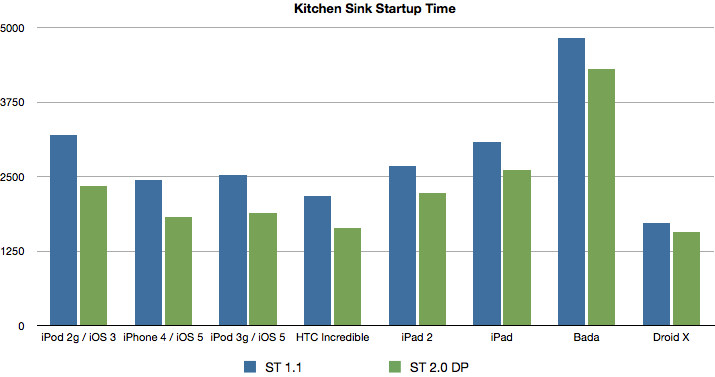
\includegraphics[width=0.8\textwidth]{figuren/sencha-touch-startup-times.png}
%   \caption{\st{} Kitchen Sink opstarttijden~\cite{SenchaInc.2013}.}
%   \label{fig:sencha_performance}
% \end{figure}

\paragraph{Aanpasbaarheid}
\label{sec:sencha-aanpasbaarheid}
Elke component binnen het raamwerk moet overerven van \code{Ext.Component}.  
Deze voorziet een attribuut \code{ui}.  
De waarde hiervan is een CSS-klasse die bepaald hoe de component er zal uitzien.  
Sencha heeft al twee CSS-klassen voorzien:  \code{light} en \code{dark}.  
Andere componenten kunnen deze lijst uitbreiden.  
Een knop kan bijvoorbeeld \code{normal},  \code{back},  \code{round},  \code{small},  \code{action} of \code{forward} als \code{ui} waarde hebben.

Het is ook mogelijk om eigen waarden voor \code{ui} te definiëren of de standaarden van Sencha aan te passen.  
SASS en Compass maken dit mogelijk door eigen CSS-bestanden aan te maken.  
SASS staat voor Syntactically Awesome Stylesheets en breidt CSS uit met variabelen,  geneste structuren, \term{mixins} en overerving~\cite{Eppstein2013}.  
\term{Mixins} groeperen enkele CSS-eigenschappen en kunnen worden hergebruikt.  
Compass is een raamwerk bovenop SASS en CSS.  
Het compileert SCSS (Sassy CSS) naar CSS-bestanden~\cite{Eppstein2013a}.        

Sencha thema's bestaan allemaal uit een set van \term{mixins}.  
Door zelf \term{mixins} te creëren of reeds bestaande te manipuleren kunnen eigen thema's gecreëerd worden en ze aan de \code{ui}-waarde van een component toegekend worden.

\paragraph{Programmeerbaarheid}
\label{sec:sencha-programeerbaarheid}
Zoals reeds aangehaald ondersteund \st{} het MVC-patroon.  
Dit patroon vermijdt lange \js{}-bestanden door ze logisch op te delen.  
Modellen groeperen velden tot een beschrijving van data-objecten, \code{Views} definiëren de weergave van componenten en controllers verbinden beide op basis van \term{events}.

In theorie zou het verschil tussen mobiele websites en applicaties enkel in de \code{Views} terug te vinden zijn.  
Echter,  dit wordt nog niet volledig ondersteund en worden aparte projecten voor deze functionaliteit gepromoot.

\paragraph{Ondersteuning browser}
\st{} steunt op de WebKit-browser \term{engine} dus moet de browser deze bevatten.  
Hoewel dit bij de meeste browsers geen probleem meer vormt, vallen toch enkele populaire browsers uit de boot.  
\st{} is bijvoorbeeld niet compatibel met FireFox Mobile en Opera Mobile~\cite{JohnEClark2012}.

Zoals reeds vermeld zijn er ook methoden voorzien om informatie op te vragen over de context die gehanteerd wordt (browser, OS, toestel, etc.).  
Verder kan \st{} ook vragen naar de ondersteuning van specifieke kenmerken (audio,  canvas,  CSS3, ...)  analoog als Modernizr.  

% TODO Tim: Senplug-incha website
Op de Senplug-incha website zijn voor sommige browsers en bijhorend besturingssystemen scorecards voorzien om hun compatibiliteit met HTLM5 en \st{} te bespreken~\cite{Inc.}.

\subsection{Motivatie}
%TODO

%%%%%%%%%%%%%%%%%%%%%%%%%%%%%%%%%%%%%%%%%%%%%%%%%%%%%%%%%%%%%%%%%%
%%%%%%%%%%%%%%%%%%%%%%%%%%%%%%%%%%%%%%%%%%%%%%%%%%%%%%%%%%%%%%%%%%

%TODO Tim: moet het eigenlijk niet Kendo UI Mobile zijn ipv Kendo UI? :)
\section{\kendo}
\label{sec:raamwerk-kendo}
% TODO Tim: idem, het zijn allemaal HTML5-raamwerken, dus ik weet niet of het nodig is om dit nog eens aan te halen
\kendo{} is een HTML5-raamwerk van de hand van Telerik.
Het bestaat uit drie luiken:  Web, Mobile en DataViz.  
Het eerste is gericht op de ontwikkeling van desktop- en mobiele applicaties,  het tweede voegt een \term{native look-and-feel} toe aan mobiele applicaties en het laatste zorgt voor datavisualisatie met HTML5- en \js{}-technologie.
%TODO Tim: MVVM uitleggen
\kendo{} is een \js{}-gedreven raamwerk met een MVVM-architectuur dat steunt op de jQuery bibliotheek.
%TODO Tim: 'in integreren aan de klantzijde'
Verder heeft de ontwikkelaar ook de mogelijkheid om eenvoudig de \term{backend} in integreren aan de klantzijde.
.NET,  PHP en JSP zijn momenteel de ondersteunde technologieën voor \term{backend} integratie.
Op het moment van schrijven is \kendo{} aan versie 2013 Q1~\cite{Telerik}. 

\subsection{Omkadering}
\label{sec:kendo-omkadering}

\paragraph{Programmeertaal}
\kendo{} kan zowel als \js{}- en opmaakgedreven beschouwd worden.  
%TODO Tim: de onderstaande zin versta ik niet zo goed
Het HTML-element dat moet omgevormd worden tot \kendo{} object moet in een HTML-bestand worden gedeclareerd.
Vervolgens kunnen data-attributen in HTML-code het element associëren met \kendo{} of kan het overeenkomstige jQuery object in \js{} het raamwerk oproepen en het element initialiseren.
%TODO Tim: GI ipv UI
Alle UI-elementen van \kendo{} Mobile kunnen met data-attributen worden opgebouwd.
\term{Widgets} van \kendo{} Web kunnen zowel met \js{} als data-attributen geïnitialiseerd worden.

Het laden van het raamwerk kan door heel \kendo{} op te roepen of enkel \kendo{} Mobile met respectievelijk \code{kendo.all.js} en \code{kendo.mobile.js}.
Elk van de drie luiken - Web, Mobile en DataViz - kan op zichzelf functioneren door hun \js{}-bestand in te laden.
Er kan wel slecht één van de drie script gelijktijdig gebruikt worden.  
Wanneer elementen uit verschillende luiken gebruikt worden, moet \code{kendo.all.js} worden gebruikt.
Een alternatieve oplossing is de keuze van het script van één luik en alle benodigde \js{}-bestanden te genereren met de \js{} Builder op \url{http://www.kendoui.com/custom-download.aspx}.
Hier kunnen de vereiste elementen geselecteerd worden en wordt het vereiste \js{}-bestand gegenereerd.
Op een analoge wijze als de \js{}-bestanden, kan de programmeur kiezen tussen verschillende \term{stylesheets}:  \code{kendo.all.css} en \code{kendo.mobile.css}.

\paragraph{Tools}
Op de \kendo{}-website staan drie webtools vermeld die Telerik aanbiedt om de programmeur te ondersteunen.
De eerste is \kendo{} Dojo~\cite{Telerika},  een interactieve leeromgeving om met \kendo{} vertrouwd te raken.
De gebruiker kan de basis van \kendo{} leren kennen met geleide handleidingen en uitvoerbare voorbeelden.
De twee andere webapplicaties zijn een ThemeBuilder voor Web en Mobile die op een grafische manier CSS-bestanden kunnen genereren~\cite{Telerikb,Telerikc}.
Voor \kendo{} Mobile kan een verschillende lay-out bepaald worden voor alle ondersteunde platformen.

\paragraph{Documentatie}
Alle documentatie kan gevonden worden op \url{http://docs.kendoui.com}~\cite{Telerikd}.
% TODO Tim: valt getting started onder een 'term'
Twee belangrijke secties binnen de documentatie zijn de API en \term{Getting Started}.
Beide kunnen op elkaar gemapt worden omdat alle objecten van \kendo{} die in de API worden aangehaald ook in een pagina onder \term{Getting Started} worden besproken.
Deze laatste probeert met meer woorden en voorbeelden uit te leggen wat het object juist inhoudt.
Verder staan er bij de documentatie nog handleidingen die complexere functionaliteit uit de doeken doet.
Ook zijn er demo's die live voorbeelden tonen samen met de code die nodig is om het voorbeeld te maken.

\paragraph{Marktadoptatie}
% TODO Tim: referentie?
Enkele van de populairste klanten van \kendo{} zijn Nikon,  Fujifilm en Symantec.

\paragraph{Licenties}
Een licentie voor \kendo{} Complete kost $\$699$ per ontwikkelaar.
Voor \term{backend} ondersteuning in PHP,  JSP of ASP.NET MVC moet $\$300$ meer betaald worden.
Hierbij zijn één jaar updates mogelijk en wordt professionele ondersteuning aangeboden met een responsetijd onder 48 uur.
Bij een licentie met \term{backend} integratie is support zelfs gegarandeerd na 24 uur.
Voor \kendo{} Web,  Mobile en DataViz bestaan ook een aparte licenties voor respectievelijk $\$399$,  $\$199$ en $\$399$.

\subsection{Code en ontwikkeling}
Zoals reeds vermeld moet de programmeur zowel \js{}- als HTML-code schrijven. 
De \js{}- en CSS-bestanden van het raamwerk moeten in de projectfolder worden gekopieerd respectievelijk in een \term{js}- en \term{styles}-map.
\kendo{} steunt op de jQuery bibliotheek en deze moet ingeladen worden voor het \kendo{} raamwerk zelf wordt aangeroepen.
De initializatie van een applicatie moet via \code{var app = new kendo.mobile.Application()}.
Hier kunnen parameters meegegeven worden die bijvoorbeeld de stijl van één platform vastlegt voor alle toestellen of het initiële scherm bepalen.

Net zoals bij \jqm{} zijn er drie strategieën om webapplicaties te maken:  volledige applicatie in één webpagina,  elk scherm in een aparte pagina of een combinatie van beide.
%TODO Tim: 'id' misschien duidelijker maken dat het om identifier gaat
De navigatie naar een scherm gebeurt op basis van de id van dat scherm.
Standaard navigeert \kendo{} naar het eerste gedefinieerde scherm van een webpagina.
Een ander scherm kan in dezelfde pagina of in een ander bestand staan.
Een lokale navigatie wordt herkend door een \term{hashtag} die voor de id van het scherm wordt geplaatst als parameter van de \code{navigate}-methode.
Navigatie naar een ander bestand kan door de bestandsnaam als parameter op te geven.

\subsection{Functionele kenmerken}
\label{sec:kendo-functioneel}
%TODO klassensysteem
\kendo{} is zowel opmaak- als \js{}-gedreven en steunt op de MVVM-architectuur.
Hierin ligt de kracht van het raamwerk,  het beïnvloedt dan ook sterk alle functionele kenmerken.

\paragraph{UI-elementen}
Formulieren volgen de de HTML5-norm. 
% TODO Tim: misschien gewoon zeggen 'versies recenter dan iOS 5.x en Android 4.x' ik snap die plus wel, maar dat is verkorte notatie voor in een tabel ofzo
Deze elementen zijn wel enkel functioneel op iOS 5.x+ en Android 4.x+.  
Het stijl van de elementen op andere platformen zal werken, maar is beperkt tot  enkel tekstinvoer~\cite{Telerike}.

Het toevoegen van knoppen kan zowel met de \code{button}-tag als met standaard hyperlinks (\code{<a>}).
Knoppen kunnen ook samengevoegd worden tot een \code{ButtonGroup}.
%TODO Tim: 'menuutje'
Dit maakt het mogelijk om gemeenschappelijke acties aan een groep van knoppen toe te kennen om bijvoorbeeld een menuutje te maken.
Een \code{TabStrip} is een alternatief waar tabs in de voettekst het scherm kunnen laten variëren.

\paragraph{View}
Schermen worden voorgesteld met \code{Views},  analoog als bij de MVC-architectuur.
Een \code{View} aanduiden gebeurt door het attribuut \code{data-role} aan \code{View} gelijk te stellen.
\code{Views} kunnen met een lay-out worden voorzien met de \code{data-layout}-tag.
Een \code{Layout} bepaalt de vormgeving van een \code{View} en kan hergebruikt worden.

Een \code{ListView} is een specifieke \code{View} voor lijsten.
De \code{data-template} kan bij lijsten de id van een sjabloon bevatten die de opmaak van de lijstelementen definieert.
% TODO Tim: 'scriptjes'
Deze sjablonen zijn specifieke \kendo{} scriptjes die HTML-tags en \js{}-code kunnen bevatten.
Ook kunnen ze verwijzen naar velden van het model dat aan de lijst is toegekend (zie infra).

Twee andere instanties van \code{Views} zijn \code{SplitView} en \code{ScrollView}.
De eerste kan het scherm in twee \code{Views} splitsen,  vaak gebruikt bij tabletapplicaties.
% TODO Tim: 'swipe' ale term
De tweede definieert een verzameling van pagina's die met een swipe bewegingen gelinkt zijn.

\paragraph{View-Model}
Het \code{View-Model} behoort tot de kern van \kendo{} en wordt \code{ObservableObject} genoemd.
Dit is een \js{}-object dat kan gebonden worden aan abonnees.
Het ondersteunt het monitoren van wijzigingen en verwittigt elke abonnee wanneer een wijziging zich voordoet.
Een \code{ObservableObject} kan aan een \code{View} worden toegekend door het in de \code{data-model}-tag te vermelden.

Er zijn verschillende bindingen	 mogelijk tussen een \code{View} en \code{ObservableObject}.
Deze wordt aangegeven in de \code{data-bind}-tag.
\kendo{} ondersteunt een binding met volgende eigenschappen:  \code{attr,  checked, clicked, custom, disabled, enabled, events, html, invisible, source, style, text, value} en \code{visible}.
Als een gebonden eigenschap wijzigt - door gebruikersinvoer of programmatisch - zal het overeenkomstige veld in het \code{ObservableObject} ook wijzigen.

\paragraph{Model}
Het \code{Model}-object erft over van \code{ObservableObject} en breidt het uit met de mogelijkheid om schema's,  velden en methoden te definiëren.  
Velden kunnen van het type \code{string, number, boolean} en \code{date} zijn.
Ook kunnen de velden verder beschreven worden door bijvoorbeeld een standaard waarde of validatie toe te voegen.
Een schema is een eigenschap van een \code{DataSource},  een \kendo{} object voor de opslag van lokale of externe data.  
Een \code{DataSource} ondersteunt alle CRUD (\term{Create, Read, Update en Delete}) operaties en het sorteren, pagineren, filteren, groeperen en aggregeren van data.
Het schema attribuut legt de structuur van de data in de \code{DataSource} vast.
Bij externe databronnen bepaalt het hoe binnenkomende data geparset moet worden om aan de opgelegde structuur te voldoen.
Een \code{Model} kan ook als waarde van het attribuut worden gezet.
Dit wil zeggen dat de bijhorende \code{DataSource} instanties zal bevatten van het toegekende \code{Model}.

% TODO Tim: ik heb tot hier de Nederlandse spelling verbeterd
\subsection{Niet-functionele kenmerken}
\label{sec:kendo-niet-functioneel}

\paragraph{Performantie}
De performantie van een \kendo{} applicatie wordt deels bepaald door de programmeur.
Deze moet er voor zorgen dat de data op het juiste moment geladen wordt.
Bij het weergeven van een \code{View} gaan drie gebeurtenissen vooraf,  respectievelijk \code{beforeShow,  init} en \code{show}.
De eerste wordt uitgevoerd voor een \code{View} zichtbaar wordt,  de tweede na initializatie en de laatste bij het tonen van een \code{View}.
Het initialiseren van een \code{View} vindt maar één keer plaats nadat de volledige applicatie geladen is.
Bij de ontwikkeling van een \code{ListView} met data van een externe databron kan best de \code{DataSource} geladen worden bij het initialiseren van de applicatie,  de lijst gemaakt worden bij de \code{init}-gebeurtenis en de lijst ververst worden wanneer bij een \code{show}-gebeurtenis.


\paragraph{Aanpasbaarheid}
\kendo{} probeert de \term{native look-and-feel} van verschillende besturingssystemen na te bootsen.
Op het moment van schrijven ondersteunt het iOS, Android, BlackBerry en WinPhone8.

Het \kendo{} pakket bevat ook tien extra thema's die een alternatieve lay-out bepalen.
Deze zijn elk nog persoonlijk aan te passen met de Mobile ThemeBuilder zoals beschreven in de sectie \ref{sec:kendo-omkadering}.

\paragraph{Programeerbaarheid}
\kendo{} is zowel JavaScipt- als opmaakgedreven.
Een kennis van zowel HTML als \js{} is vereist om met dit raamwerk aan de slag te kunnen.
Het raamwerk is gebouwd op de jQuery Core en maakt dus vaak van jQuery \term{selectors} gebruik.
Ook kan een AJAX verzoek met jQuery syntax geformuleerd worden om externe data op te halen voor een \code{DataSource}.

\paragraph{Browserondersteuning}
Zoals reeds vermeld herkent \kendo{} het platform waarop de applicatie wordt uitgevoerd.
De lay-out van de applicatie zal de \term{native look-and-feel} van het besturingssysteem vervolgens nabootsen.
Ondersteunde systemen zijn iOS, Android, BlackBerry en WinPhone8.

Alle widgets, zoals gebruikt in het raamwerk, ondersteunen \term{progressive enhancement}.
Oudere browsers kunnen zo bestaande inhoud en functionaliteit raadplegen met \term{native} HTML types indien bepaalde elementen niet worden ondersteund.
Ook de HTML5 formulierelementen worden opgebouwd met \term{progressive enhancement}.

\subsection{Motivatie}
%TODO

%%%%%%%%%%%%%%%%%%%%%%%%%%%%%%%%%%%%%%%%%%%%%%%%%%%%%%%%%%%%%%%%%%
%%%%%%%%%%%%%%%%%%%%%%%%%%%%%%%%%%%%%%%%%%%%%%%%%%%%%%%%%%%%%%%%%%

%TODO: verder uitschrijven, maar dat zal blijken uit mijn implementatie
\section{\lungo}
\label{sec:raamwerk-lungo}

\lungo{} is een opmaakgedreven raamwerk waarbij versie~1.0 uitkwam in 2011~\cite{TapQuo2011}.
Het raamwerk wordt onderhouden door TapQuo dat een Spaans bedrijf is, gespecialiseerd rond mobiele gebruikerservaring~\cite{TapQuo2013a}.
Analoog met \jqm{} is \lungo{} afhankelijk van een \js{}-bibliotheek, namelijk \quo{}.
\lungo{} biedt vooral GI-elementen aan, maar daarnaast zijn er ook \term{wrappers} voor cache, opslag en SQL beschikbaar~\cite{TapQuo2013}.
Net zoals \jqm{} wordt geen programmeerstijl zoals MVC afgedwongen.
Op het moment van schrijven zit \lungo{} aan versie~2.1~\cite{TapQuo2013}.

\subsection{Omkadering}
\paragraph{Programmeertaal}
Net zoals bij \jqm{} is er niets meer nodig dan kennis over HTML, CSS en \js{}.
De GI-elementen worden geschreven in HTML en aangeduid aan de hand van CSS-klassen en \code{data-*}-attributen

\paragraph{Tools}
Er worden geen specifieke tools door TapQuo aangeboden om de ontwikkeling te versnellen.
Wel kan er gebruik worden gemaakt van Twitter Bower die helpt om de bestanden van het \lungo{}-raamwerk tezamen met de \quo{}-bibliotheek te beheren~\cite{Twitter2013}.
Dit is bij \jqm{} niet mogelijk doordat \jqm{} geen geldige component is van Bower.

\paragraph{Documentatie}
De documentatie start op \exturl{lungo.tapquo.com/howto/prototype/} waar getoond wordt hoe het geraamte van een typische \lungo{}-applicatie er uitziet.
Daarnaast zijn er nog 8 andere hoofdstukken die de aangeboden GI-elementen en API uitleggen.
Op de documentatiepagina's is altijd eerst de broncode te zien.
Er kan dan boven de broncode op een knop geklikt worden, waarna een levensecht voorbeeld wordt getoond.

\paragraph{Marktadoptatie}
TODO (mail sturen)

\paragraph{Licenties}
Het raamwerk wordt onder de GPLv3-licentie vrijgegeven.
Een commerciële versie is mogelijk.

\subsection{Code en ontwikkeling}
Zoals gezegd wordt een \lungo{}-applicatie geprogrammeerd vanuit geannoteerde HTML-code door middel van CSS-klasses.
Net zoals \jqm{} wordt er geen programmeerstijl zoals MVC afgedwongen.

Om de verschillende schermen te scheiden wordt gebruik gemaakt van \code{<article>}- en \code{<section>}-tags die specifiek zijn voor HTML5.
Analoog wordt ook voor de kop- en voettekst de \code{<header>}- en \code{<footer>}-tags gebruikt.
Hierdoor is het duidelijk dat \lungo{} ten opzichte van \jqm{} volledig gebruik maakt van de nieuwste HTML5-tags.

\lungo{} biedt de mogelijkheid om de verschillende schermen op afzonderlijke pagina's op te slaan en daarna asynchroon op te halen.
In tegenstelling tot \jqm{} dient enkel wat binnen de \code{<body>}-tag staat, opgeslaan te worden.
Bij \jqm{} dient telkens ook de volledige \code{<head>}-tag op iedere pagina herhaald te worden.

\subsection{Functionele kenmerken}
De documentatiepagina is opgedeeld in 9 groepen die hieronder kort worden aangehaald.

\begin{enumerate}

\item \textbf{Prototype } 
Hierop worden GI-elementen, navigatie, formulieren, scrollen, lijsten en data-attributen aangehaald. 
Opmerkelijk is de directe ondersteuning door het raamwerk bij het naar beneden trekken van een lijst waarbij de data automatisch wordt herladen.

\item \textbf{Core }
Hier worden functies aangehaald die het raamwerk zelf intern gebruik.
Een voorbeeld hiervan is de \code{Lungo.Core.isMobile()}-functie die controleert of de applicatie in een mobiele omgeving wordt uitgevoerd.

\item \textbf{Data }
Zoals aangehaald in de inleiding biedt het raamwerk \term{wrappers} voor cache, opslag en SQL.
De ontwikkelaar dient dus zelf geen \code{if-then-else}-constructies op te stellen of een bepaald kenmerk ondersteund wordt of niet, het raamwerk neemt dat onder de moterkap voor zijn rekening.

\item \textbf{DOM }
Het manipuleren van de DOM gebeurt door de \quo{}-bibliotheek.
Hierbij wordt gerefereerd naar de documentatie op \exturl{quojs.tapquo.com}.

\item \textbf{Element }
Toevoegen van een telbubbel, vooruitgangsbalk, laadbalk, automatisch herladen bij het naar beneden trekken van lijst en een fotocarousel zijn mogelijk vanuit \js{}. 

\item \textbf{Notification }
Er worden standaard verschillende dialoogvensters aangeboden voor fout-, succes- en infomeldingen.
 
\item \textbf{Routing }
Hier wordt uitgebreid ingegaan op de navigatie doorheen de applicatie vanuit \js{}.

\item \textbf{Service }
Versturen van HTTP-oproepen kan zonder enig probleem vanuit het \lungo{}—raamwerk.

\item \textbf{View }
Hier worden \js{}-methoden aangeboden om het uitzicht binnen een \code{<article>} te bepalen.
 
\end{enumerate}

\subsection{Niet-functionele kenmerken}
\paragraph{Performantie}
Een voordeel, dat zal moeten blijken in hoofdstuk~\ref{chap:evaluatie}, is dat de \js{}-bibliotheek waarop \lungo{} steunt, geoptimaliseerd is voor mobiel gebruik.
Dit is in tegenstelling tot jQuery die ook methodes aanbiedt voor desktopgebruikers.
Hierdoor bevat \quo{} enkel de nodige code, waardoor het bestand kleiner zal zijn in grootte en dus ook sneller wordt gedownload. 

\paragraph{Aanpasbaarheid}
\label{sec:sencha-aanpasbaarheid}
Standaard ziet een \lungo{}-applicatie er goed uit qua lay-out.
TapQuo biedt zelf geen tools aan om de kleuren of het uitzicht van de applicatie te veranderen.
Hierdoor zal een ontwikkelaar zelf aangewezen zijn om eigen CSS-code te schrijven.

\paragraph{Programmeerbaarheid}
\label{sec:sencha-programeerbaarheid}
\lungo{} dwingt geen enkel ontwerppatroon af.
Voor de echte functionaliteit wordt beroep gedaan op \js{} en meer bepaald op \quo{}. 
Ook deze dwingt geen ontwerppatroon af.

\paragraph{Ondersteuning browser}
TapQuo geeft aan op hun website dat ze ondersteuning bieden voor iOS, Android, Blackberry en FirefoxOS.
Verder halen ze aan dat ze een consistente ervaring willen hebben van een gemaakte applicatie van mobiele apparaten, tv's tot desktopapparaten.


\subsection{Motivatie}
%TODO

%%%%%%%%%%%%%%%%%%%%%%%%%%%%%%%%%%%%%%%%%%%%%%%%%%%%%%%%%%%%%%%%%%
%%%%%%%%%%%%%%%%%%%%%%%%%%%%%%%%%%%%%%%%%%%%%%%%%%%%%%%%%%%%%%%%%%

\section{Tabel}
\label{sec:raamwerken-tabel}

\pgfplotstabletypeset[
  col sep=comma,
  string type,
  header=true,
  columns={Criterium,jQM,ST,Kendo,Lungo},
  columns/Criterium/.style={column name={}, column type={c}},  
  columns/jQM/.style={column name=\textbf{\jqm}, column type={c}},
  columns/ST/.style={column name=\textbf{\st}, column type={c}},
  columns/Kendo/.style={column name=\textbf{\kendo}, column type={c}},
  columns/Lungo/.style={column name=\textbf{\lungo}, column type={c}},
  every head row/.style={
    before row=\toprule,
    after row=\midrule},
  every last row/.style={
    after row=\bottomrule}
]{tabellen/raamwerken.csv}

